\begin{enumerate}[label={},font=\normalfont,leftmargin=1.15cm,labelwidth=1.0cm,labelsep=0.15cm,itemindent=0pt,listparindent=0pt,itemsep=\baselineskip,parsep=0pt,topsep=0pt]
\item[2.2.1] If $A^2=4A+3I$ and $A^{-1}=xA+yI$, find $x+y$.

\begin{multicols}{4}
\begin{enumerate}
\setlength{\itemsep}{0pt}
    \item $-1$
    \item $1$
    \item $\frac53$
    \item $7$\nobreak\hfill\mbox{(12,2026)}
\end{enumerate}
\end{multicols}



\vspace{0.6em}\par\solution


Let $v\ne0$ be an eigenvector of $A$ with eigenvalue $\lambda$. Applying $A^2=4A+3I$ to $v$ gives $\lambda^2-4\lambda-3=0$, so the possible eigenvalues are $\lambda_+=2+\sqrt7$ and $\lambda_-=2-\sqrt7$.
\par\noindent\hfill\mbox{\textit{(\ref{formula-2-1-13})}}\par
They are distinct. For the intended non-scalar case, both occur. Applying $A^{-1}=xA+yI$ to eigenvectors for these eigenvalues gives
\[
\frac1{\lambda_+}=x\lambda_++y,\qquad \frac1{\lambda_-}=x\lambda_-+y.
\]
The eigenvalue equation also gives $1/\lambda_\pm=(\lambda_\pm-4)/3$. Subtracting the two equations yields
\[
x=\frac{1/\lambda_+-1/\lambda_-}{\lambda_+-\lambda_-}=\frac13,\qquad y=\frac1{\lambda_+}-x\lambda_+=-\frac43.
\]
Therefore, $x+y=-1$, so the correct answer is \textbf{a)}.

\textit{If $A$ is a scalar multiple of $I$, the values of $x$ and $y$ are not uniquely determined; the question implicitly assumes the non-scalar case.}
\item[2.2.2] If a square matrix $A$ satisfies $A^2=A$ and $(I-A)^3=xA+I$, find $x$.\nobreak\hfill\mbox{(12,2026)}



\vspace{0.6em}\par\solution


Since $A^2=A$, its minimal polynomial divides $t(t-1)$, which has distinct roots; hence $A$ is diagonalizable. For some invertible matrix $P$, write
\[
A=P\begin{bmatrix}I_r&0\\0&0\end{bmatrix}P^{-1},\qquad I-A=P\begin{bmatrix}0&0\\0&I_{n-r}\end{bmatrix}P^{-1}.
\]
\par\noindent\hfill\mbox{\textit{(\ref{formula-2-1-14})}}\par
Thus $(I-A)^3=P\begin{bmatrix}0&0\\0&I_{n-r}\end{bmatrix}P^{-1}=I-A$. Comparing with $xA+I$ gives $(x+1)A=0$, so for $A\ne0$, $\boxed{x=-1}$. If $A=0$, the equation holds for every $x$; the stated answer assumes $A$ is nonzero.

\item[2.2.3] If $B(\operatorname{adj}B)=\begin{bmatrix}\frac13&0&0\\0&\frac13&0\\0&0&\frac13\end{bmatrix}$, find $\det(B^{-1})$.

\begin{multicols}{4}
\begin{enumerate}
\setlength{\itemsep}{0pt}
    \item $\frac13$
    \item $3$
    \item $-3$
    \item $9$\nobreak\hfill\mbox{(12,2026)}
\end{enumerate}
\end{multicols}



\vspace{0.6em}\par\solution


Since $B(\operatorname{adj}B)=\frac13I_3$ is nonsingular, $B$ is nonsingular. Let $v\ne0$ be an eigenvector of $B$ with eigenvalue $\lambda$. Then $\lambda\ne0$ and, using $\operatorname{adj}B=\det(B)B^{-1}$,
\[
\operatorname{adj}B\,v=\frac{\det(B)}{\lambda}v,\qquad B(\operatorname{adj}B)v=\det(B)v.
\]
But the given equation also gives $B(\operatorname{adj}B)v=\frac13v$. Since $v\ne0$, $\det(B)=\frac13$, and hence $\det(B^{-1})=\frac1{\det(B)}=\boxed{3}$, option \textbf{b)}. The Python code checks the determinant value from the given product.
\par\noindent\hfill\mbox{\textit{(\ref{formula-2-1-1})}}\par\begin{lstlisting}[frame=single, basicstyle=\rmfamily, escapeinside={(*@}{@*)}]
(*@\makebox[\dimexpr\linewidth-2\fboxsep-2\fboxrule\relax][c]{codes/2.2.3.py}@*)
\end{lstlisting}

\item[2.2.4] Find $k$ such that $f(x)=\begin{cases}x^2\sin(1/x),&x\ne0,\\k(x+1),&x=0\end{cases}$ is continuous.\nobreak\hfill\mbox{(12,2026)}



\vspace{0.6em}\par\solution


At $x=0$, the second branch gives $f(0)=k$. For $x\ne0$, since $-1\le\sin(1/x)\le1$ and $x^2\ge0$,
\[
-x^2\le x^2\sin(1/x)\le x^2.
\]
Both bounds tend to $0$ as $x\to0$. By the squeeze theorem, $\lim_{x\to0}x^2\sin(1/x)=0$. Thus continuity requires $k=0$. The figure plots the function together with the bounding curves $y=-x^2$ and $y=x^2$.
\par\noindent\hfill\mbox{\textit{(\ref{formula-2-1-3}, \ref{formula-2-1-15})}}\par\begin{lstlisting}[frame=single, basicstyle=\rmfamily, escapeinside={(*@}{@*)}]
(*@\makebox[\dimexpr\linewidth-2\fboxsep-2\fboxrule\relax][c]{codes/2.2.4.py}@*)
\end{lstlisting}
\begin{figure}[H]\centering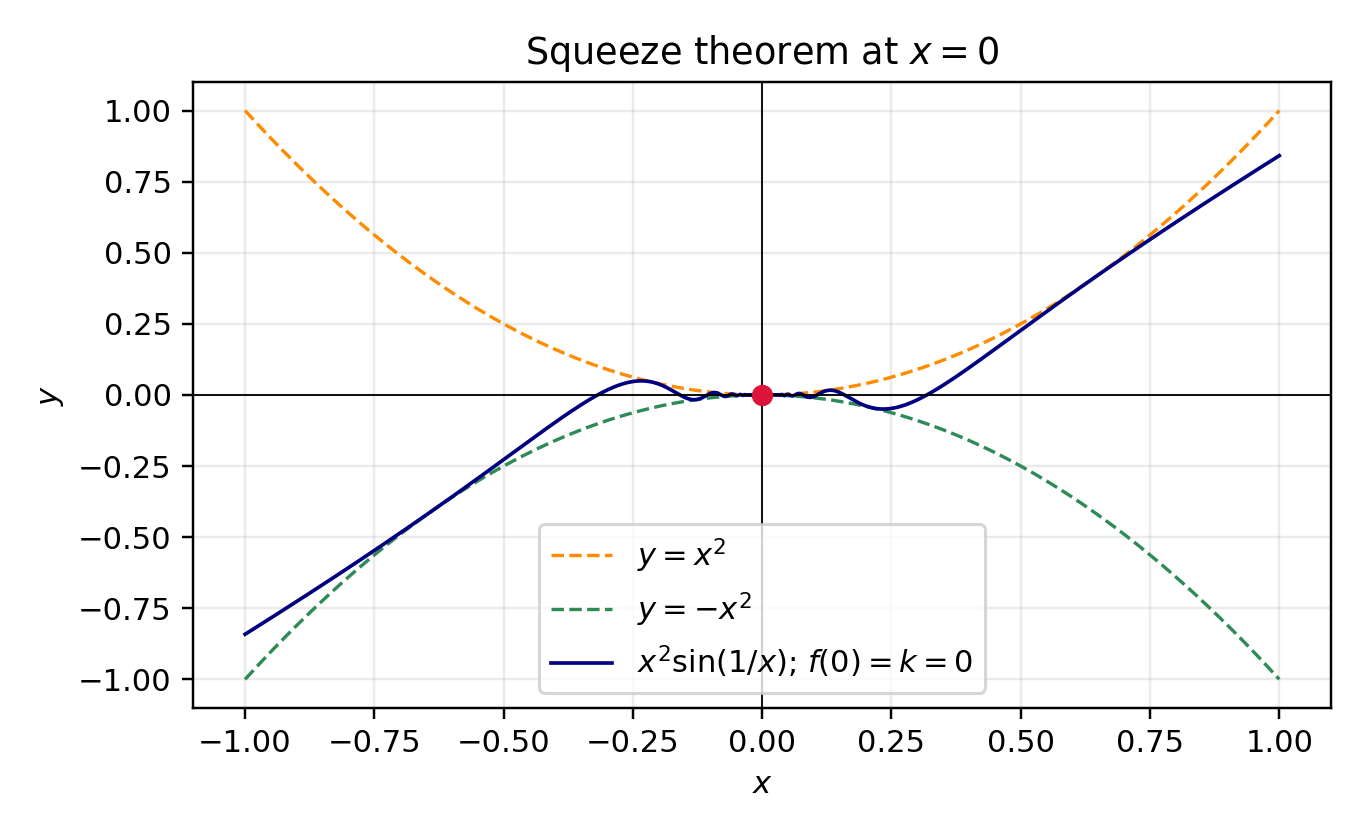
\includegraphics[width=0.68\linewidth]{figs/2.2.4.png}\caption{The function approaches $0$ as $x$ approaches $0$.}\end{figure}

\item[2.2.5] Evaluate $\int_{-1}^{1}(1-|x|)\,dx$ by identifying the matching option:

\begin{multicols}{2}
\begin{enumerate}
\setlength{\itemsep}{0pt}
    \item $2\int_0^1(1+x)\,dx$
    \item $2\int_{-1}^0(1+x)\,dx$
    \item $0$
    \item $2\int_{-1}^0(1-x)\,dx$\nobreak\hfill\mbox{(12,2026)}
\end{enumerate}
\end{multicols}



\vspace{0.6em}\par\solution


Use the nodes $x_0=-1$, $x_1=0$, and $x_2=1$ ($h=1$), where the function values are $0$, $1$, and $0$. The composite trapezoidal rule gives
\[
T=\frac{h}{2}\bigl(f(x_0)+2f(x_1)+f(x_2)\bigr)
=\frac12(0+2+0)=1.
\]
This is exact because $f(x)=1-|x|$ is linear on each half of the interval.

The same area accumulation can be written as a difference equation. Let $A_j$ be the accumulated area through $x_j$, with $A_0=0$. For $j=0,1$,
\[
A_{j+1}-A_j=\frac{h}{2}\bigl(f(x_j)+f(x_{j+1})\bigr).
\]
Thus $A_1-A_0=\frac12$ and $A_2-A_1=\frac12$, giving $A_2=1$. Also, on $[-1,0]$, $f(x)=1+x$; by symmetry the integral is $2\int_{-1}^0(1+x)\,dx$, which is option \textbf{b)}.\par\noindent\hfill\mbox{\textit{(\ref{formula-2-1-6}, \ref{formula-2-1-16})}}\par\begin{lstlisting}[frame=single, basicstyle=\rmfamily, escapeinside={(*@}{@*)}]
(*@\makebox[\dimexpr\linewidth-2\fboxsep-2\fboxrule\relax][c]{codes/2.2.5.py}@*)
\end{lstlisting}
\begin{figure}[H]\centering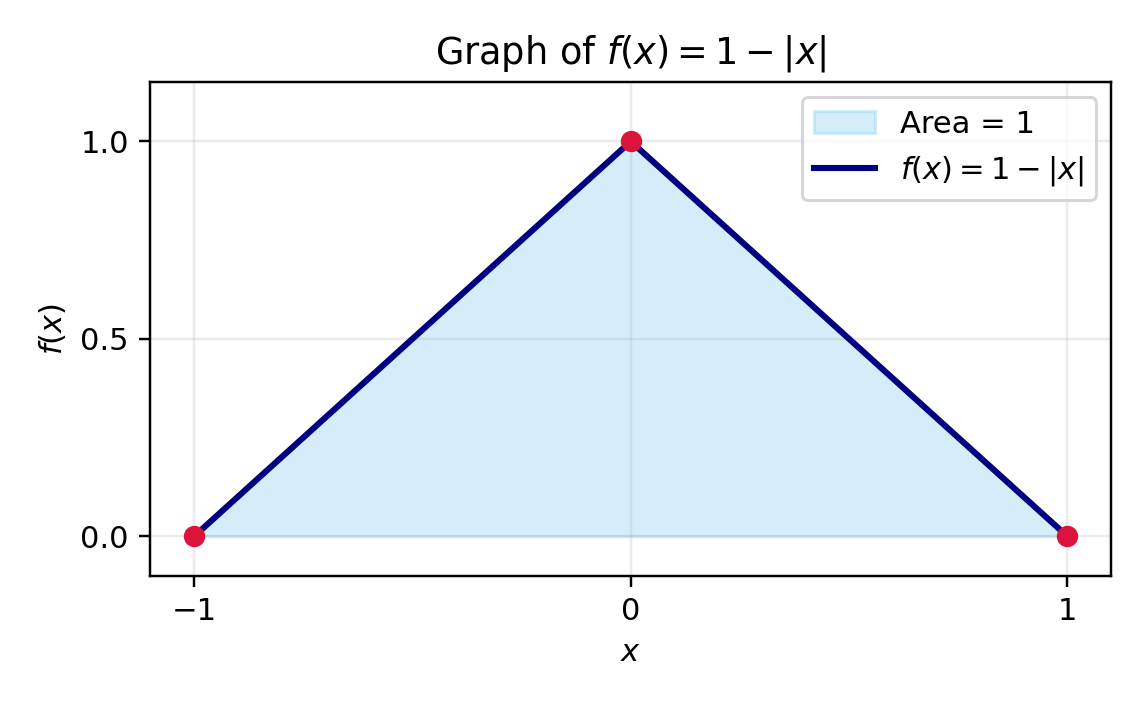
\includegraphics[width=0.40\linewidth]{figs/2.2.5.png}\caption{Graph of $f(x)=1-|x|$ on $[-1,1]$.}\end{figure}

\item[2.2.6] For the circle $x^2+y^2=9$, identify the integral for the shaded cap above $y=1$.

\begin{multicols}{2}
\begin{enumerate}
\setlength{\itemsep}{0pt}
    \item $\int_1^3\sqrt{9-y^2}\,dy$
    \item $2\int_1^3\sqrt{9-y^2}\,dy$
    \item $\int_0^3\sqrt{9-x^2}\,dx$
    \item $2\int_0^3\sqrt{9-x^2}\,dx$\nobreak\hfill\mbox{(12,2026)}
\end{enumerate}
\end{multicols}



\vspace{0.6em}\par\solution


At height $y$, the cap's width is $w(y)=2\sqrt{9-y^2}$ for $1\le y\le3$. Thus $A=\int_1^3w(y)\,dy$, which is option \textbf{b)}. CVXPY approximates this area with midpoint slices by maximizing $\Delta y\sum_iw_i$ subject to $0\le w_i\le2\sqrt{9-y_i^2}$; the code compares the result with all four choices.\par\noindent\hfill\mbox{\textit{(\ref{formula-2-1-5}, \ref{formula-2-1-10}, \ref{formula-2-1-17})}}\par\begin{lstlisting}[frame=single, basicstyle=\rmfamily, escapeinside={(*@}{@*)}]
(*@\makebox[\dimexpr\linewidth-2\fboxsep-2\fboxrule\relax][c]{codes/2.2.6.py}@*)
\end{lstlisting}
\begin{figure}[H]\centering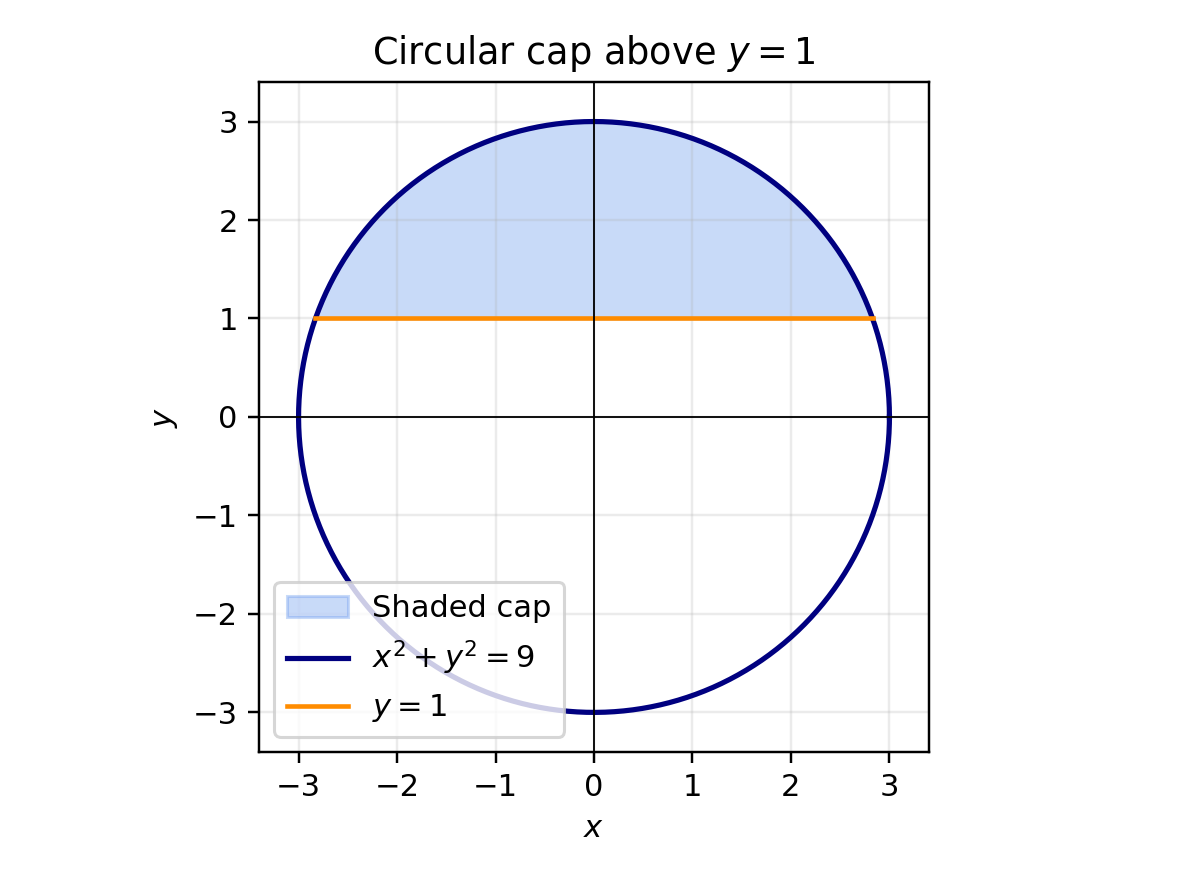
\includegraphics[width=0.48\linewidth]{figs/2.2.6.png}\caption{Circle $x^2+y^2=9$ and the cap above $y=1$.}\end{figure}

\item[2.2.7] If $(\vec a+\vec b)\cdot(\vec a-\vec b)=198$ and $|\vec a|=10|\vec b|$, select the true statement.

\begin{multicols}{2}
\begin{enumerate}
\setlength{\itemsep}{0pt}
    \item $|\vec a|=\sqrt2$
    \item $|\vec b|=\sqrt2$
    \item $|\vec b|=10\sqrt2$
    \item $|\vec a|=10/\sqrt2$\nobreak\hfill\mbox{(12,2026)}
\end{enumerate}
\end{multicols}



\vspace{0.6em}\par\solution


Using $(\vec a+\vec b)\cdot(\vec a-\vec b)=|\vec a|^2-|\vec b|^2$, let $r=|\vec b|\ge0$. Since $|\vec a|=10r$,
\[
100r^2-r^2=198,\qquad r^2=2.
\]
The reduced convex problem is
\[
\text{maximize }r\quad\text{subject to }r\ge0,\quad r^2\le2.
\]
Its largest feasible value is $r=\sqrt2$, so $|\vec b|=\sqrt2$ and the answer is \textbf{b)}. CVXPY solves this reduced scalar problem.
\par\noindent\hfill\mbox{\textit{(\ref{formula-2-1-9})}}\par\begin{lstlisting}[frame=single, basicstyle=\rmfamily, escapeinside={(*@}{@*)}]
(*@\makebox[\dimexpr\linewidth-2\fboxsep-2\fboxrule\relax][c]{codes/2.2.7.py}@*)
\end{lstlisting}

\item[2.2.8] Find the sub-interval(s) of $(0,\pi/2)$ in which $f(x)=\tan x-4x$ is increasing.\nobreak\hfill\mbox{(12,2026)}



\vspace{0.6em}\par\solution


$f'(x)=\sec^2x-4>0$ precisely when $\cos x<1/2$ on this domain, so the critical point is $x=\pi/3$. Therefore $f$ is increasing on $\boxed{(\pi/3,\pi/2)}$. The Python code uses bisection to locate the zero of $f'(x)$ numerically and plots $f$, shading the interval where it increases.
\par\noindent\hfill\mbox{\textit{(\ref{formula-2-1-3}, \ref{formula-2-1-4}, \ref{formula-2-1-18})}}\par\begin{lstlisting}[frame=single, basicstyle=\rmfamily, escapeinside={(*@}{@*)}]
(*@\makebox[\dimexpr\linewidth-2\fboxsep-2\fboxrule\relax][c]{codes/2.2.8.py}@*)
\end{lstlisting}
\begin{figure}[H]\centering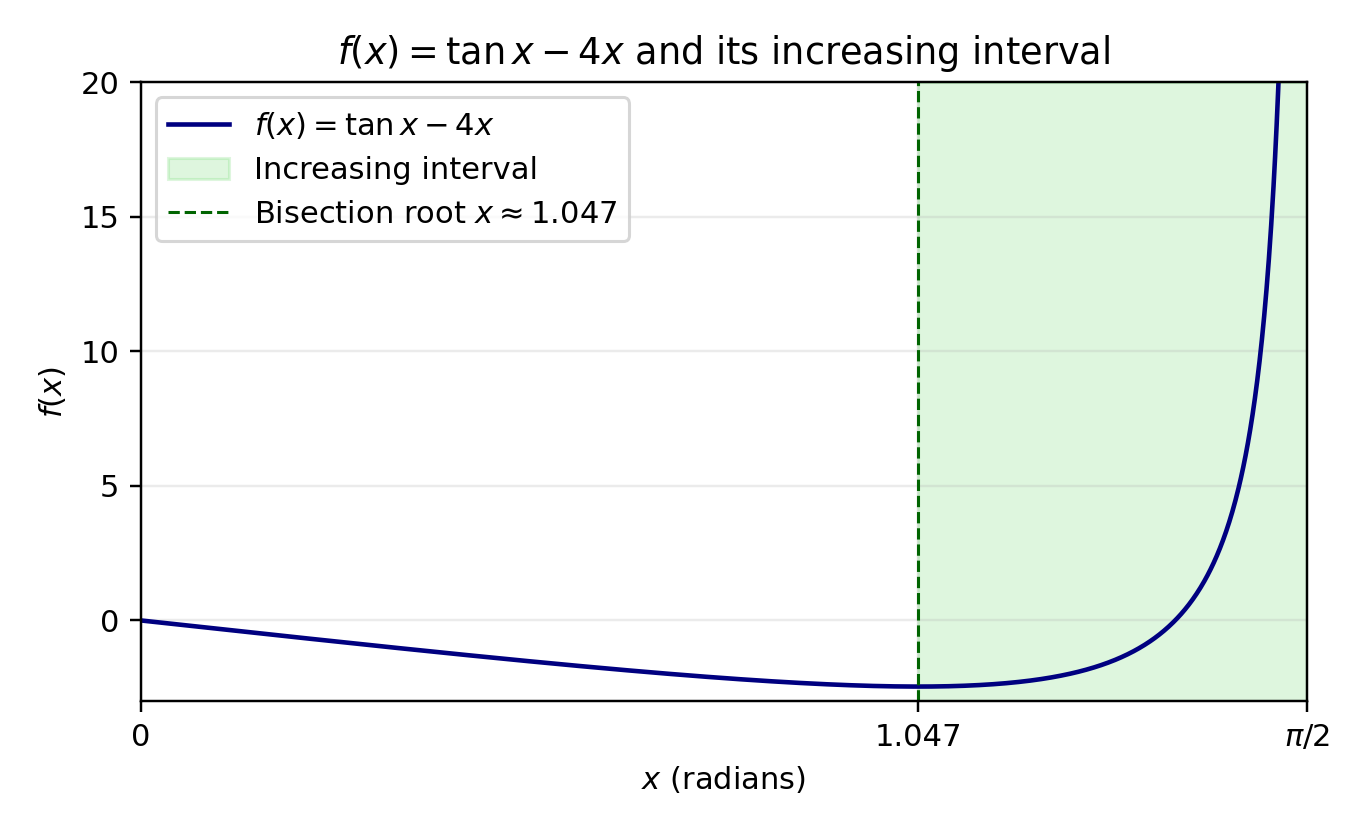
\includegraphics[width=0.68\linewidth]{figs/2.2.8.png}\caption{The function rises on the shaded interval.}\end{figure}

\item[2.2.9] For unit vectors $\vec a,\vec b$, if $|\vec a+2\vec b|=|2\vec a-\vec b|$, find the angle between them.\nobreak\hfill\mbox{(12,2026)}



\vspace{0.6em}\par\solution


Let $c=\vec a\cdot\vec b$. Since $|\vec a|=|\vec b|=1$, their Gram matrix is
\[
G=\begin{bmatrix}1&c\\c&1\end{bmatrix}.
\]
The squared lengths are
\[
|\vec a+2\vec b|^2=
\begin{bmatrix}1&2\end{bmatrix}G\begin{bmatrix}1\\2\end{bmatrix}=5+4c,
\qquad
|2\vec a-\vec b|^2=
\begin{bmatrix}2&-1\end{bmatrix}G\begin{bmatrix}2\\-1\end{bmatrix}=5-4c.
\]
The given equality implies $5+4c=5-4c$, so $c=0$. Thus $\cos\theta=\vec a\cdot\vec b=0$, and the angle is $\boxed{90^\circ}$.\par\noindent\hfill\mbox{\textit{(\ref{formula-2-1-9}, \ref{formula-2-1-19})}}\par

\item[2.2.10]
(a) If $\frac{x-3}{1}=\frac{1-y}{1}=\frac{z+2}{p}$ and $\frac{2-x}{3}=\frac{y+1}{5}=\frac{z+56}{2p}$ are perpendicular, find $p$.\\
\textbf{OR}\\
(b) Find the vector equation of the line through the origin perpendicular to both $\vec r=2\hat i-\hat j+2\hat k+\lambda(3\hat i+4\hat j+2\hat k)$ and $\vec r=\mu(\hat i-\hat j+\hat k)$.\nobreak\hfill\mbox{(12,2026)}



\vspace{0.6em}\par\solution


(a) The direction vectors are $(1,-1,p)$ and $(-3,5,2p)$. Their dot product is $2p^2-8$, so $\boxed{p=\pm2}$.\\
(b) Let the required direction be $(a,b,c)$. Perpendicularity gives $3a+4b+2c=0$ and $a-b+c=0$. Taking $b=1$ gives $a=-6$, $c=7$. Thus the line is $\boxed{\vec r=t(-6\hat i+\hat j+7\hat k)}$. The Python code verifies both dot products and plots the vectors without using a cross product.
\par\noindent\hfill\mbox{\textit{(\ref{formula-2-1-9}, \ref{formula-2-1-11})}}\par\begin{lstlisting}[frame=single, basicstyle=\rmfamily, escapeinside={(*@}{@*)}]
(*@\makebox[\dimexpr\linewidth-2\fboxsep-2\fboxrule\relax][c]{codes/2.2.10.py}@*)
\end{lstlisting}
\begin{figure}[H]\centering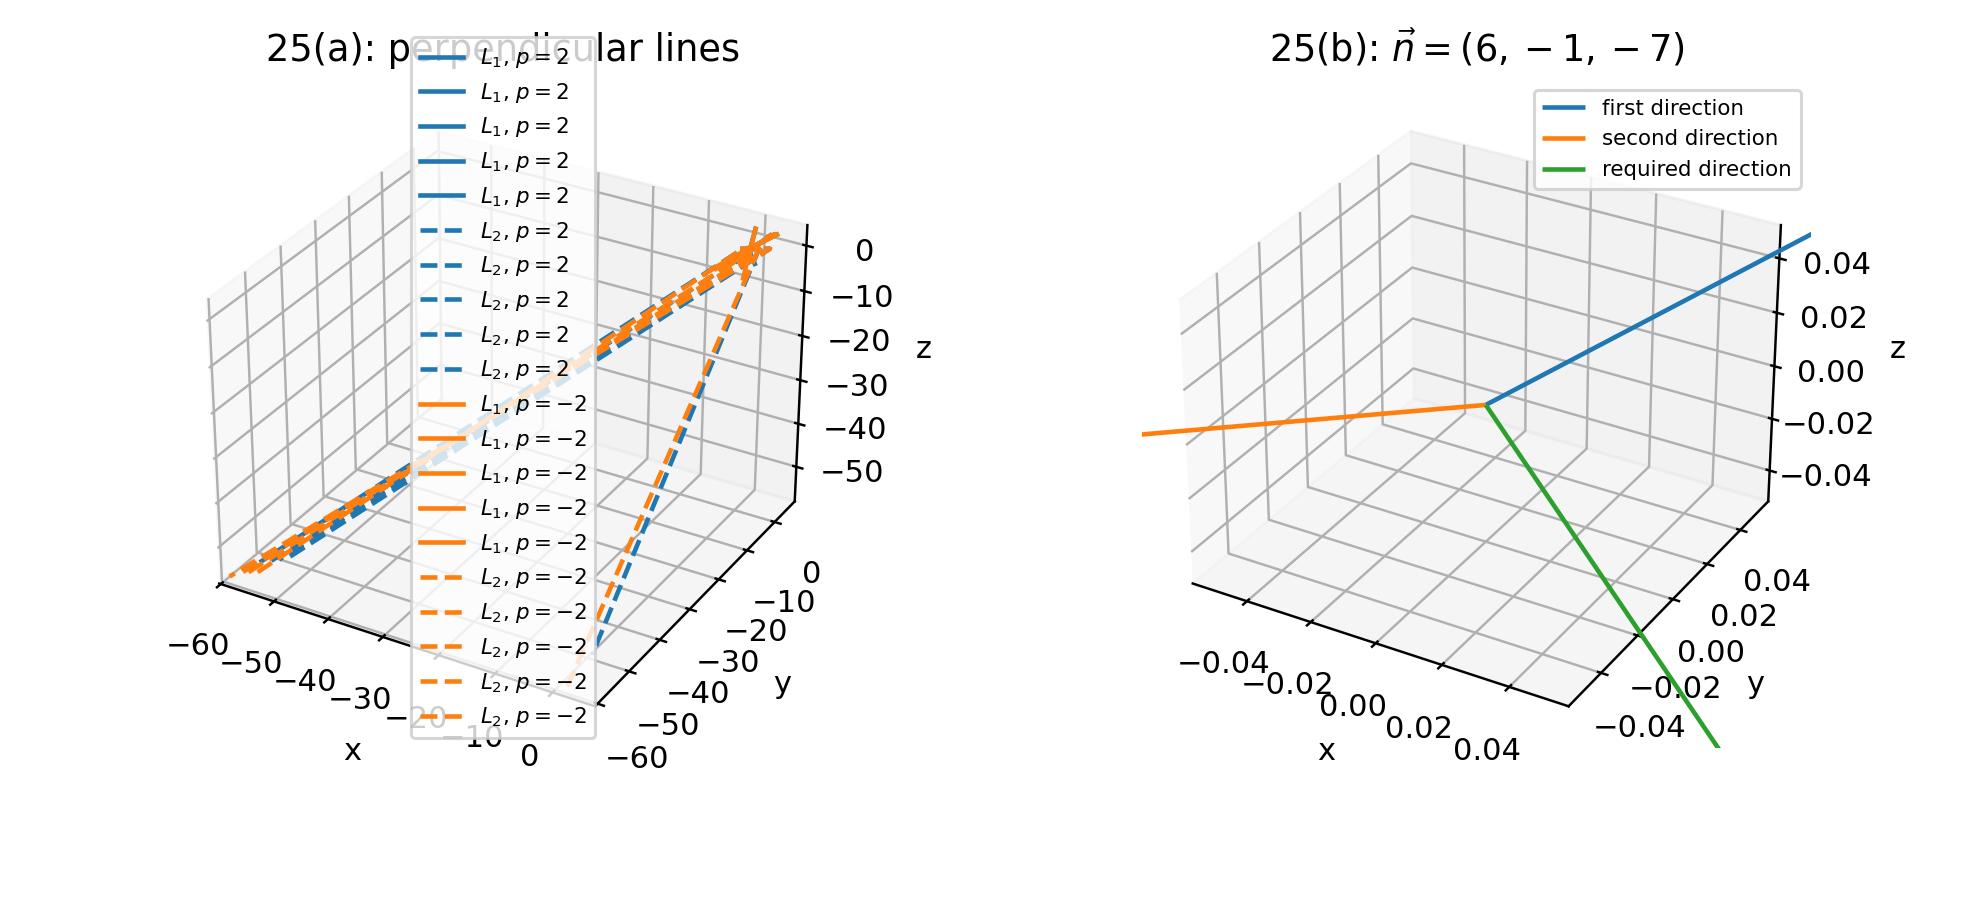
\includegraphics[width=0.75\linewidth]{figs/2.2.10.png}\caption{Direction diagrams for the two alternatives in Question 25.}\end{figure}

\item[2.2.11] Robotic knee replacement surgery has a $90\%$ success rate. For three independent surgeries, find the probability that (i) exactly one succeeds, and (ii) at most two succeed.\nobreak\hfill\mbox{(12,2026)}



\vspace{0.6em}\par\solution


Let $X$ be the number of successful surgeries. Independence gives the PMF
\[
p_X(k)=\binom{3}{k}(0.9)^k(0.1)^{3-k},\qquad k=0,1,2,3.
\]
Its values are
\[
\begin{array}{c|cccc}
k&0&1&2&3\\\hline
p_X(k)&0.001&0.027&0.243&0.729
\end{array}.
\]
(i) $P(X=1)=p_X(1)=\boxed{0.027}$. (ii) $P(X\le2)=p_X(0)+p_X(1)+p_X(2)=0.001+0.027+0.243=\boxed{0.271}$.\par\noindent\hfill\mbox{\textit{(\ref{formula-2-1-8}, \ref{formula-2-1-20})}}\par

\item[2.2.12] Show that $f:\mathbb R\to\mathbb R$, $f(x)=\frac{x}{\sqrt{1+x^2}}$, is one-one but not onto.\nobreak\hfill\mbox{(12,2026)}



\vspace{0.6em}\par\solution

$f'(x)=(1+x^2)^{-3/2}>0$, so $f$ is strictly increasing and therefore one-one. Also $|f(x)|<1$ for every real $x$, and its range is $(-1,1)$, so it is not onto $\mathbb R$. The plot illustrates the range.
\par\noindent\hfill\mbox{\textit{(\ref{formula-2-1-3}, \ref{formula-2-1-18})}}\par
\begin{lstlisting}[frame=single, basicstyle=\rmfamily, escapeinside={(*@}{@*)}]
(*@\makebox[\dimexpr\linewidth-2\fboxsep-2\fboxrule\relax][c]{codes/2.2.12.py}@*)
\end{lstlisting}
\begin{figure}[H]\centering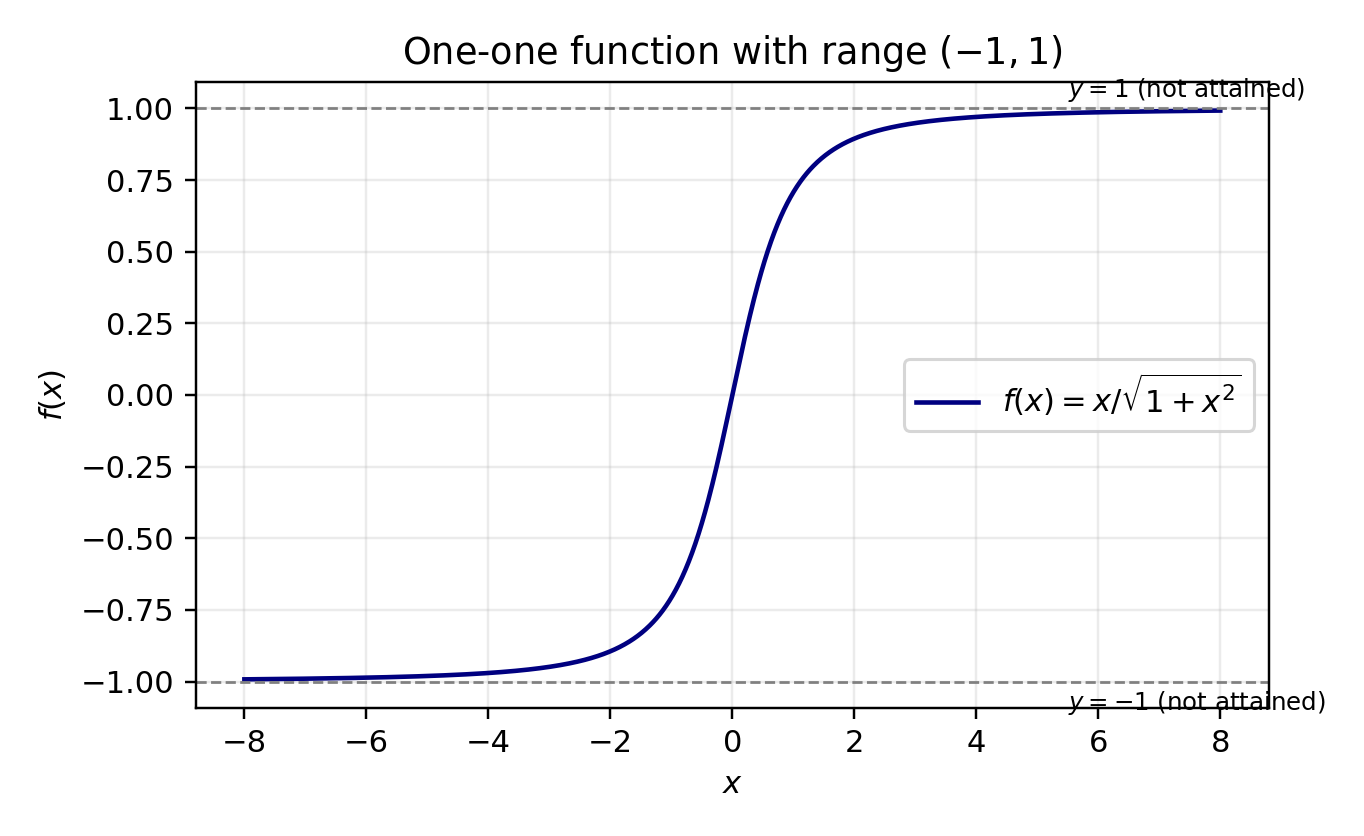
\includegraphics[width=0.68\linewidth]{figs/2.2.12.png}\caption{The function is strictly increasing and approaches, but never reaches, $\pm1$.}\end{figure}

\item[2.2.13] Solve graphically: maximize $Z=600x+400y$ subject to $x+2y\le12$, $4x+5y\ge20$, $2x+y\le12$, and $x,y\ge0$.\nobreak\hfill\mbox{(12,2026)}



\vspace{0.6em}\par\solution


The feasible vertices are $(0,4),(0,6),(4,4),(6,0),(5,0)$. Evaluating $Z$ gives $1600,2400,4000,3600,3000$, respectively. Thus $\boxed{Z_{\max}=4000}$ at $(4,4)$. The Python code uses CVXPY to solve the linear program and uses CoordGeo to plot the constraints and label the feasible vertices.
\par\noindent\hfill\mbox{\textit{(\ref{formula-2-1-10})}}\par\begin{lstlisting}[frame=single, basicstyle=\rmfamily, escapeinside={(*@}{@*)}]
(*@\makebox[\dimexpr\linewidth-2\fboxsep-2\fboxrule\relax][c]{codes/2.2.13.py}@*)
\end{lstlisting}
\begin{figure}[H]\centering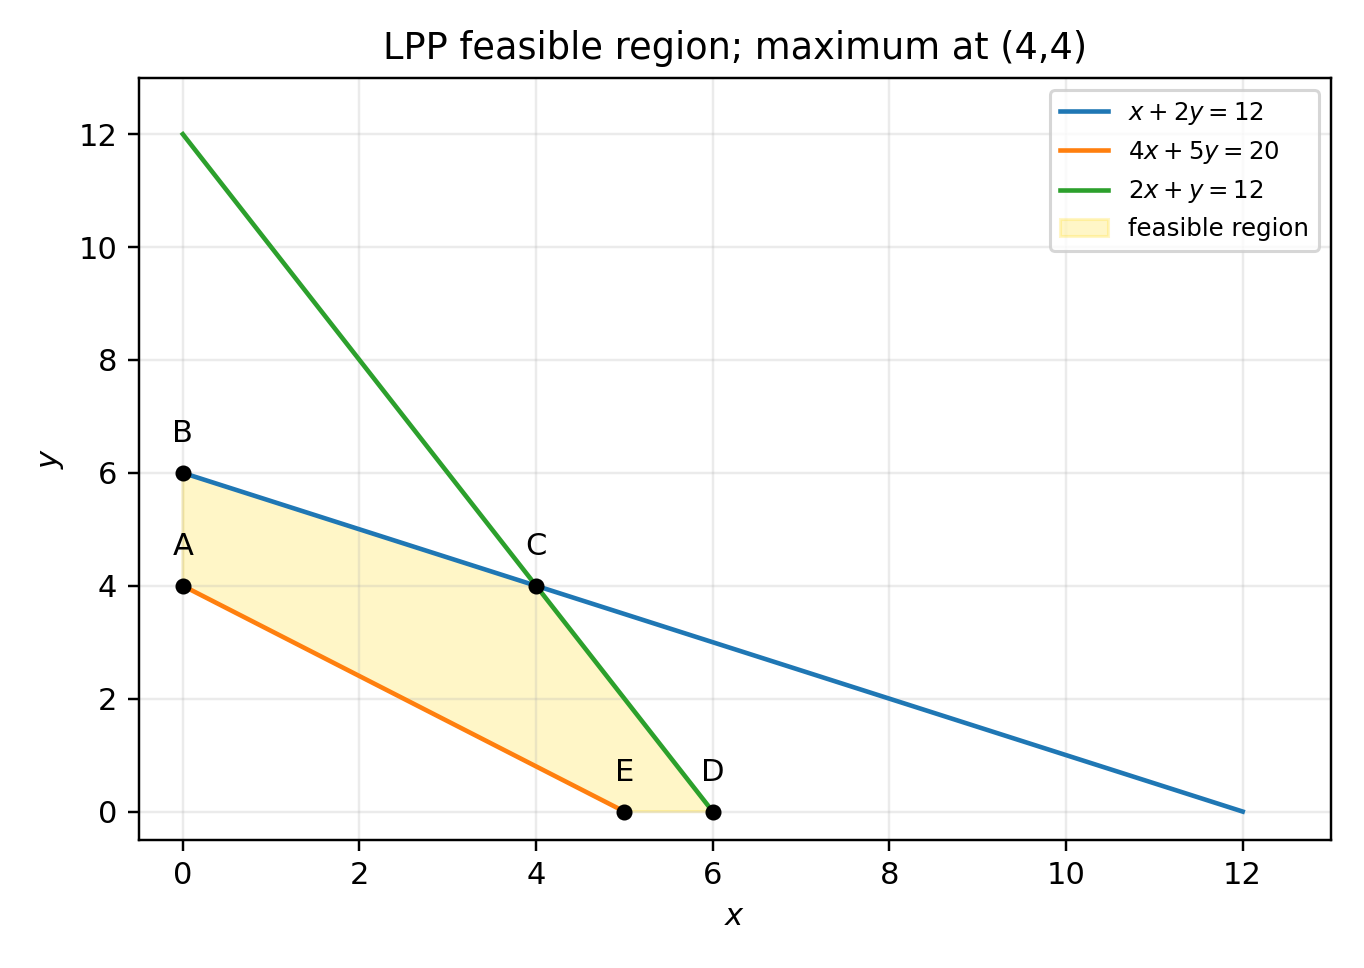
\includegraphics[width=0.68\linewidth]{figs/2.2.13.png}\caption{The shaded feasible region has its maximum at $(4,4)$.}\end{figure}

\item[2.2.14]
\noindent(a) A showroom gives 60 vouchers of Rs. 1,000 and Rs. 500. The number of Rs. 1,000 vouchers plus three times the number of Rs. 500 vouchers is 100. Form the equations and find the counts by the matrix method.\\
\textbf{OR}\\
\noindent(b) Given $P=\begin{bmatrix}2&-1\\3&4\end{bmatrix}$, $Q=\begin{bmatrix}5&2\\7&4\end{bmatrix}$ and $R=\begin{bmatrix}2&5\\3&8\end{bmatrix}$, find $S$ such that $PQ-RS=O$.\nobreak\hfill\mbox{(12,2026)}



\vspace{0.6em}\par\solution


\noindent(a) Let $x,y$ denote the two voucher counts. Then $x+y=60$, $x+3y=100$. Subtracting the first equation from the second gives $2y=40$, so $y=20$ and $x=40$. Thus there are $\boxed{40}$ Rs. 1,000 vouchers and $\boxed{20}$ Rs. 500 vouchers. The Python code solves the augmented system by Gaussian elimination.\par\noindent\hfill\mbox{\textit{(\ref{formula-2-1-21})}}\\
\noindent(b) First compute $PQ=\begin{bmatrix}3&0\\43&22\end{bmatrix}$ and solve $RS=PQ$ by Gaussian elimination. This gives
\begin{equation*}
\boxed{S=\begin{bmatrix}-191&-110\\77&44\end{bmatrix}}.
\tag*{(\ref{formula-2-1-1}, \ref{formula-2-1-21})}\end{equation*}
\begin{lstlisting}[frame=single, basicstyle=\rmfamily, escapeinside={(*@}{@*)}]
(*@\makebox[\dimexpr\linewidth-2\fboxsep-2\fboxrule\relax][c]{codes/2.2.14a.py}@*)
\end{lstlisting}
\begin{lstlisting}[frame=single, basicstyle=\rmfamily, escapeinside={(*@}{@*)}]
(*@\makebox[\dimexpr\linewidth-2\fboxsep-2\fboxrule\relax][c]{codes/2.2.14b.py}@*)
\end{lstlisting}

\item[2.2.15]
(a) Write the lines $\frac{x+3}{-3}=\frac{y-1}{1}=\frac{z-5}{5}$ and $\frac{x+1}{-1}=\frac{2-y}{-2}=\frac{z-5}{5}$ in vector form and check whether they intersect.\\
\textbf{OR}\\
(b) A square has opposite sides along $\vec r=(1,2,-4)+\lambda(2,3,6)$ and $\vec r=(3,3,-5)+\mu(2,3,6)$. If the other pair has direction ratios $(-3,6,p)$, find the square's area and $p$.\nobreak\hfill\mbox{(12,2026)}



\vspace{0.6em}\par\solution


(a) The vector forms are $\vec r=(-3,1,5)+\lambda(-3,1,5)$ and $\vec r=(-1,2,5)+\mu(-1,2,5)$. At $\lambda=\mu=-1$, both pass through $(0,0,0)$, so they intersect there.\\
(b) The separation of the parallel lines is $\sqrt{293}/7$, so the square's area is $\boxed{293/49}$. Perpendicular adjacent side directions require $(2,3,6)\cdot(-3,6,p)=0$, giving $\boxed{p=-2}$. The Python code computes the line intersection, square side length, area, and $p$, then plots both configurations using CoordGeo.
\par\noindent\hfill\mbox{\textit{(\ref{formula-2-1-9}, \ref{formula-2-1-11})}}\par\begin{lstlisting}[frame=single, basicstyle=\rmfamily, escapeinside={(*@}{@*)}]
(*@\makebox[\dimexpr\linewidth-2\fboxsep-2\fboxrule\relax][c]{codes/2.2.15.py}@*)
\end{lstlisting}
\begin{figure}[H]\centering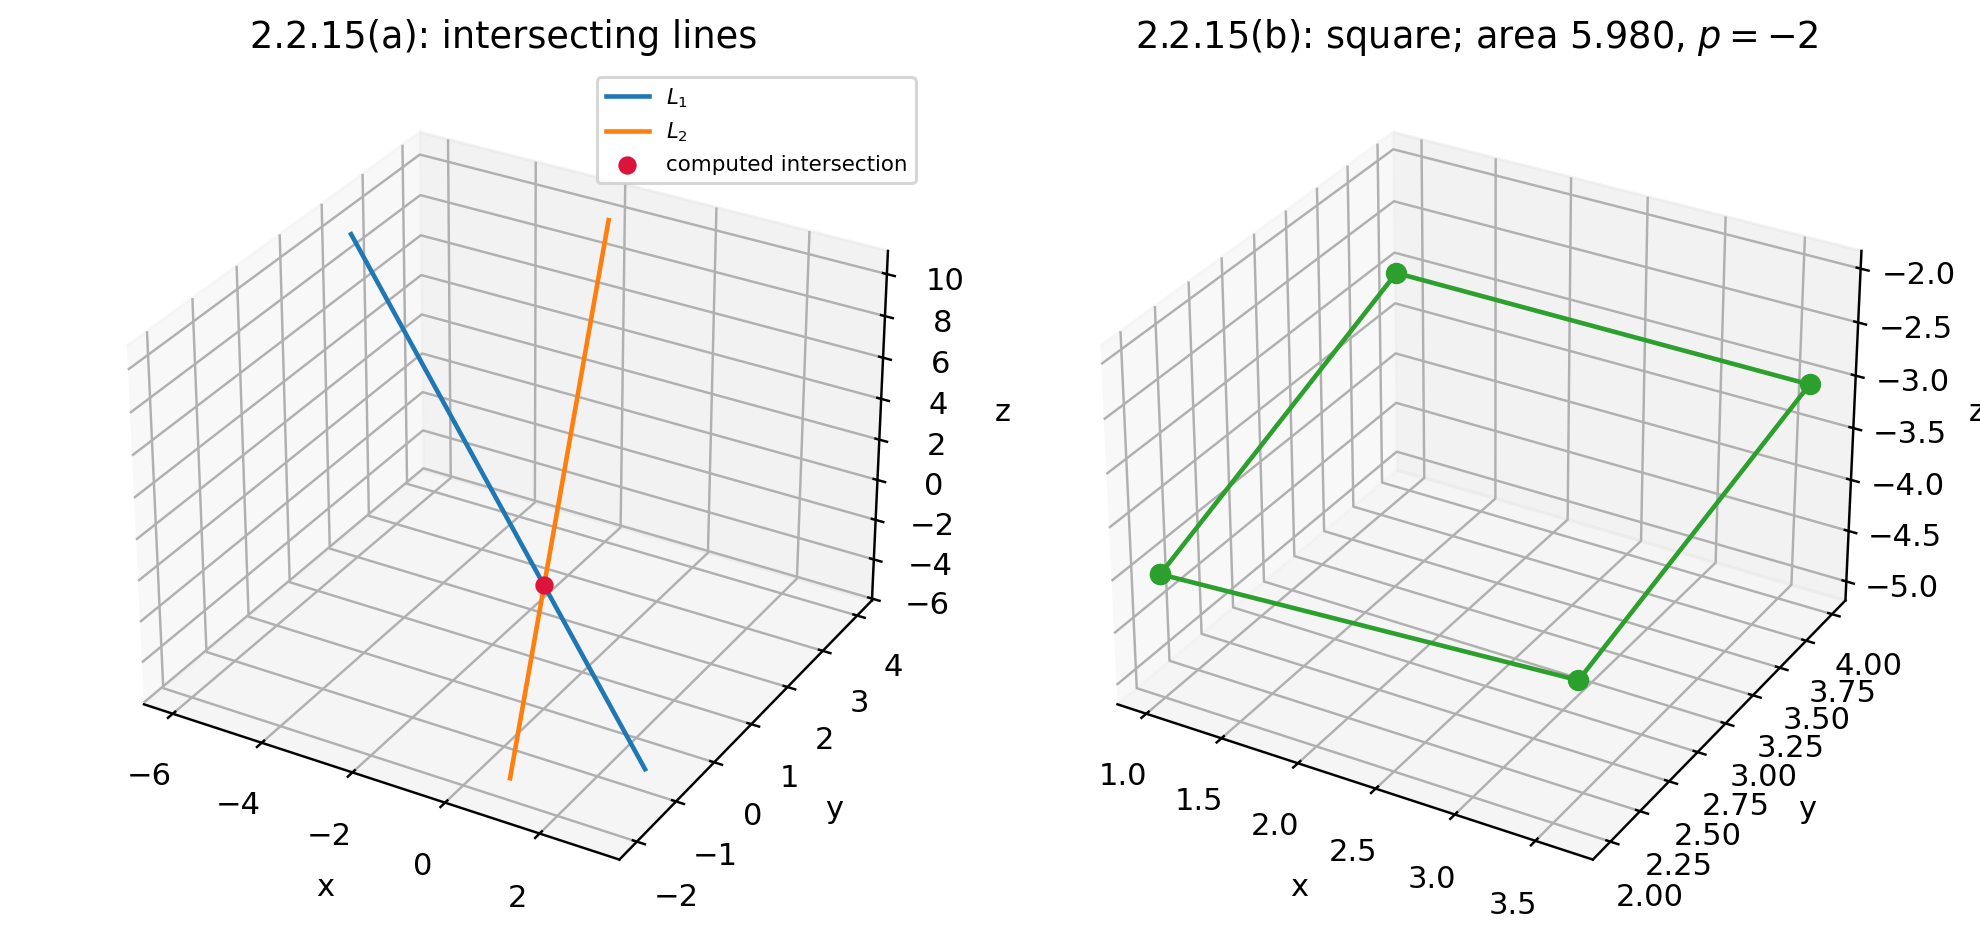
\includegraphics[width=0.75\linewidth]{figs/2.2.15.png}\caption{The two line configurations and the square between parallel lines.}\end{figure}

\item[2.2.16] Two vertical poles of heights $22$ m and $16$ m stand on opposite sides of a $20$ m road. Ladders from a point $R$, $x$ m from the shorter pole, reach their tops. (i) Express $p(x)=l_1+l_2$. (ii) Find $p'(x)$. (iii)(a) Find $x$ minimizing $l_1^2+l_2^2$. \textbf{OR} (b) if both poles are $16$ m tall, find the position minimizing the sum of squared ladder lengths.\nobreak\hfill\mbox{(12,2026)}



\vspace{0.6em}\par\solution


The horizontal distances from $R$ to the $22$ m and $16$ m poles are $20-x$ and $x$, respectively. Hence
\begin{equation*}
\begin{aligned}
l_1(x)&=\sqrt{484+(20-x)^2}, & l_2(x)&=\sqrt{256+x^2},\\
p(x)&=l_1+l_2=\sqrt{484+(20-x)^2}+\sqrt{256+x^2},\\
p'(x)&=-\frac{20-x}{\sqrt{484+(20-x)^2}}+\frac{x}{\sqrt{256+x^2}}.
\end{aligned}
\tag*{(\ref{formula-2-1-3}, \ref{formula-2-1-4})}\end{equation*}
For (a),
\[
l_1^2+l_2^2=484+(20-x)^2+256+x^2=2(x-10)^2+940,
\]
so the minimum occurs at $\boxed{x=10\text{ m}}$.
For (b), if both poles are $16$ m tall, the sum of squared ladder lengths is
\[
[256+(20-x)^2]+[256+x^2]=2(x-10)^2+712,
\]
which is minimized when $\boxed{x=10\text{ m}}$, the midpoint of the road. The CVXPY code independently minimizes the squared-length objective for both height configurations and prints the optimal position and minimum value.
\par\begin{lstlisting}[frame=single, basicstyle=\rmfamily, escapeinside={(*@}{@*)}]
(*@\makebox[\dimexpr\linewidth-2\fboxsep-2\fboxrule\relax][c]{codes/2.2.16.py}@*)
\end{lstlisting}

\item[2.2.17] Of students taking an entrance examination, $40\%$ are dropouts and $60\%$ are regular students. The pass rates are $5\%$ for dropouts and $10\%$ for regular students. Find (i) the probability a student is regular, (ii) the probability a dropout fails, (iii)(a) given a student passed, the probability they are not a dropout, \textbf{OR} (b) given a student failed, the probability they were regular.\nobreak\hfill\mbox{(12,2026)}



\vspace{0.6em}\par\solution


Let $X$ denote the student's type ($D$: dropout, $R$: regular), and $Y$ the result ($S$: pass, $F$: fail). Their joint PMF is
\[
p_{X,Y}(x,y)=P(X=x)P(Y=y\mid X=x),
\]
The joint PMF and its marginals are
\[
\begin{array}{c|cc|c}
X\backslash Y & S & F & p_X(x)\\\hline
D & 0.02 & 0.38 & 0.40\\
R & 0.06 & 0.54 & 0.60\\\hline
p_Y(y) & 0.08 & 0.92 & 1
\end{array}.
\]
Using the joint PMF and its marginals,
\begin{align*}
\text{(i)}\quad&P(X=R)=0.06+0.54=\boxed{0.60}.\\
\text{(ii)}\quad&P(Y=F\mid X=D)=\frac{0.38}{0.40}=\boxed{0.95}.\\[2pt]
\text{(iii)(a)}\quad&P(X=R\mid Y=S)=\frac{0.06}{0.08}=\boxed{\frac34}.\\[2pt]
\text{(iii)(b)}\quad&P(X=R\mid Y=F)=\frac{0.54}{0.92}=\boxed{\frac{27}{46}}.
\tag*{(\ref{formula-2-1-8}, \ref{formula-2-1-12}, \ref{formula-2-1-20})}\end{align*}

\item[2.2.18] A triangular park has vertices $A(0,4)$, $B(-2,0)$ and $C(3,0)$, with $O=(0,0)$. Find (i) the equation of $AB$, (ii) the equation of $AC$, and (iii)(a) the area of $OAC$ by integration, \textbf{OR} (b) the area of $AOB$ by integration.\nobreak\hfill\mbox{(12,2026)}



\vspace{0.6em}\par\solution


Using the slopes from the given vertices,
\[
AB:\ y=2x+4,\qquad AC:\ y=4-\frac43x.
\]
For (a), split $[0,3]$ into $n$ equal steps of width $h=3/n$, with $x_k=kh$. Let $A_0=0$ and accumulate each rectangle by the difference equation
\[
A_{k+1}-A_k=h\left(4-\frac43x_k\right).
\]
Summing the recurrence gives
\[
\begin{aligned}
A_n&=\frac3n\sum_{k=0}^{n-1}\left(4-\frac{4k}{n}\right)=6+\frac6n\longrightarrow 6,\\
\therefore\quad \operatorname{area}(OAC)&=\boxed{6\text{ square units}}.
\end{aligned}
\]
\newpage
For (b), take $h=2/n$, $x_k=-2+2k/n$, and $B_0=0$. The corresponding recurrence and sum are
\[
B_{k+1}-B_k=h(2x_k+4),\qquad
B_n=\frac2n\sum_{k=0}^{n-1}\frac{4k}{n}=4\left(1-\frac1n\right)\longrightarrow4,
\]
so $\operatorname{area}(AOB)=\boxed{4\text{ square units}}$. These accumulated rectangle sums converge to the definite integrals in the question. The plot code uses CoordGeo's line generator and point-labeling function.
\par\noindent\hfill\mbox{\textit{(\ref{formula-2-1-5}, \ref{formula-2-1-17})}}\par
\begin{lstlisting}[frame=single, basicstyle=\rmfamily, escapeinside={(*@}{@*)}]
(*@\makebox[\dimexpr\linewidth-2\fboxsep-2\fboxrule\relax][c]{codes/2.2.18.py}@*)
\end{lstlisting}
\begin{figure}[H]\centering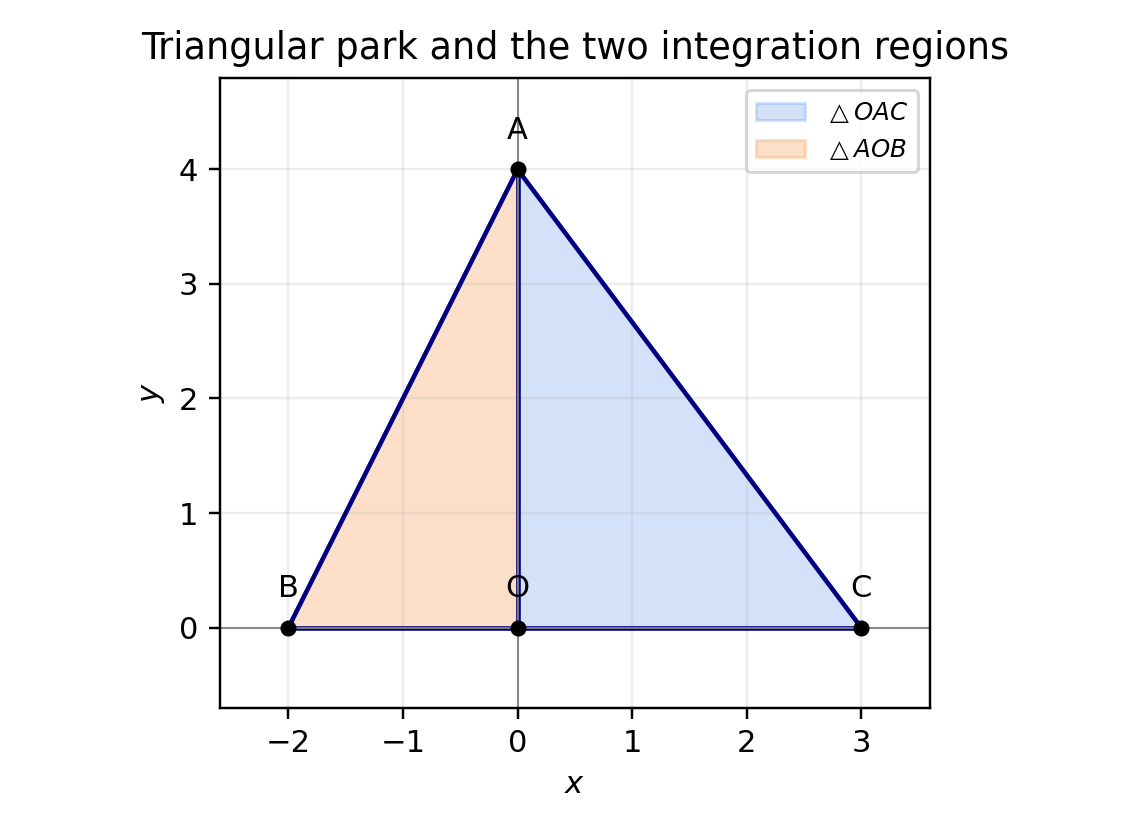
\includegraphics[width=0.55\linewidth]{figs/2.2.18.png}\caption{The shaded regions $OAC$ and $AOB$ are evaluated by integration.}\end{figure}
\end{enumerate}
